\section{Auswertung}
\label{sec:Auswertung}
\subsection{Bestimmung der Metalle über die Dichte}
Die Metalle lassen sich über ihr Volumen V und ihre Masse m bestimmen (Abb.1).
Im Vergleich zu dem Literaturwert von  zeigt sich, dass beide Stäbe aus Messing bestehen.
\begin{table}[h]
  \centering
  \label{tab:lit}
  \begin{tabular}{ c c c c c c }
    \toprule
    {$\text{Stab}$}
   &{$l \,\, \text{in} \, [m]$}
   &{$d \,\, \text{in} \, [m]$}
   %&{$h \, in \, [m]$}
   &{$V \,\, \text{in} \, [m^3]$}
   &{$m \,\, \text{in} \, [kg]$}
   &{$\rho \,\, \text{in} \, [\frac{kg}{m^3}]$} \\
    \midrule
     {$\text{eckig}$}&60&1&60&502.4 & 8.367 \\
     {$\text{rund}$}&60.05&1&15\pi&394.4 & 8.361 \\
    \bottomrule
  \end{tabular}
  \caption{Dichte der Metalle}
\end{table}










\subsection{Eckiger Stab, einseitige Einspannung}
\begin{figure}
  \centering
  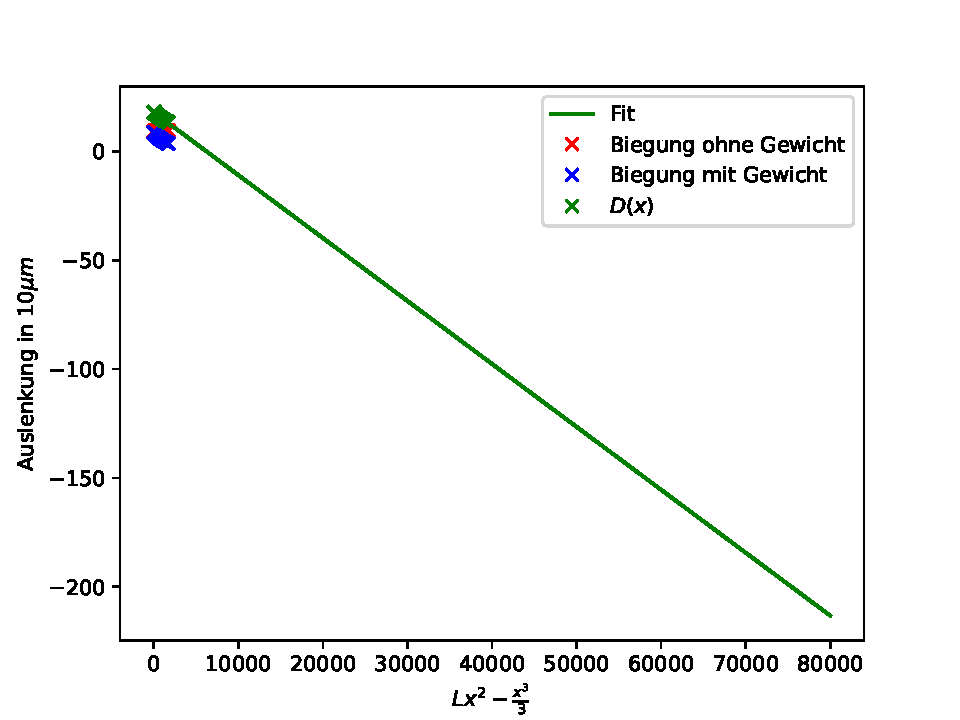
\includegraphics{build/plot1.pdf}
  \caption{Plot1.}
  \label{fig:plot1}
\end{figure}

\subsection{Runder Stab, einseitige Einspannung}
\begin{figure}
  \centering
  \includegraphics{build/plot2.pdf}
  \caption{Plot2.}
  \label{fig:plot2}
\end{figure}

\subsection{Runder Stab, beidseitige Einspannung}
\begin{figure}
  \centering
  \includegraphics{build/plot3.pdf}
  \caption{Plot3.}
  \label{fig:plot3}
\end{figure}
